\documentclass{article} % For LaTeX2e
\usepackage{nips14submit_e,times}
\usepackage{hyperref}
\usepackage{url}
\usepackage[pdftex]{graphicx}	
\usepackage{float}
\usepackage[caption = false]{subfig}
%\documentstyle[nips14submit_09,times,art10]{article} % For LaTeX 2.09

\title{Visualization of Community Structure in Scientific Networks}

\author{
Yuan Huang \\
Department of Physics\\
University of Massachusetts, Amherst\\
Amherst, MA, 01002 \\
\texttt{yuanh@physics.umass.edu} \\
}

% The \author macro works with any number of authors. There are two commands
% used to separate the names and addresses of multiple authors: \And and \AND.
%
% Using \And between authors leaves it to \LaTeX{} to determine where to break
% the lines. Using \AND forces a linebreak at that point. So, if \LaTeX{}
% puts 3 of 4 authors names on the first line, and the last on the second
% line, try using \AND instead of \And before the third author name.

\newcommand{\fix}{\marginpar{FIX}}
\newcommand{\new}{\marginpar{NEW}}
\nipsfinalcopy % Uncomment for camera-ready version

\begin{document}

\maketitle

\section{Introduction}
\label{intro}

Detecting community structure is an important task in the field of complex networks. Community structure in a network refers to that the vertices in networks are often found to cluster into different groups with a large number of within-group edges and a small number of edges between groups. In this paper, we focus on the community structure in the citation networks of academic articles. The analysis of the underlying community structure in citation networks provides numerous benefits for the development of the research field, including building a foundation for future research through the acknowledgement of past research activities; identifying gaps in research for researchers and students; improving the integration between theory and practice, and so on~\cite{phys_rev, OLED, learning_analytics, sustain}. On the other hand, finding clusters in network-structured data is a fundamental problem that has many applications in social networks and other related fields. 

In this project, we will apply two recently proposed clustering methods\cite{bottom_up, new_method} to detect the community structure in Physical Review citation network. The first method is a bottom-up agglomerative clustering method based on modularity maximization, which is computationally more efficient than the previous divisive approach ~\cite{phys_rev}. The other clustering method is based on non-binary hierarchical tree with overlapping clusters~\cite{new_method}, which has been tested for some well-known benchmark network datasets, but not in a large-scale citation network before. We test the robustness of these two methods and check the significance of our results using the modularity measure. We apply both algorithms to the Physical Review citation network to resolve its major communities and the connections between them. We also visualize the structure of the individual communities.

%%%%Add results

\section{Related Works}
\label{related}
The analysis of citation and co-authorship network has been performed for many research fields, such as organic LED~\cite{OLED}, learning analysis~\cite{learning_analytics}, sustainable science~\cite{sustain}, and so on. The study of the community structure has been attracting more and more interest in the field of scientific network study. In recent years, a growing number of clustering algorithms for categorical data have been proposed to study the community structure of the scientific networks~\cite{Newman_divisive, bottom_up, new_method, Newman_evaluation,  method_review, Newman_algorithm}. 

In 2008, Leicht and Newman~\cite{Newman_divisive} proposed a general divisive hierarchical clustering algorithm for network. The method try to maximize the modularity of the graph using the eigenvalues and eigenvectors of the modularity matrix. By iteratively divide each group into subgroups according to the leading eigenvectors of the modularity matrix, the algorithm can achieve the clustering that maximize the global modularity. 

At the same year, Blondel et. al.~\cite{bottom_up} proposed a highly efficient agglomerative clustering algorithm. Here each network node is initially assigned to a unique community. Then, the algorithm iteratively groups the pair of nodes that maximizes the increase of the global modularity into the same community, until a maximal modularity is achieved. This algorithm is computationally more efficient than the previous divisive approach but has the disadvantage of requiring more memory. 

In 2010, Chen and Redner~\cite{phys_rev} investigated the community structure of physics subfields in the citation network of well-cited Physical Review Publications (with more than 100 citations). In their paper, they applied the divisive hierarchical algorithm based on modularity maximization~\cite{Newman_divisive} to identify community within networks and performed analysis on the major communities. They also examined communities decade by decade and found a small number of significant links between communities that are widely separated in time. 

In 2011, Zhao and Zhang~\cite{new_method} proposed a new clustering method for detecting community structures. In this method, individuals and their relationships are denoted by weighted graphs, then the graph density gives a better quantity depict of whole correlation among individuals in a community, so that a reasonable clustering output can be presented. By constructing a non-binary hierarchical tree of clusters, this method has two important features: one is that the hierarchical tree is much smaller that clearly highlights meaningful clusters; the other one is the clusters can overlap with each other which does reflect the complexity of our real world.

%%%Expand on the three papers

\section{Methodology}
\label{method}

Various clustering algorithms have been proposed in the literature in many different scientific disciplines. These clustering algorithms can be broadly divided into two groups: (i) hierarchical method and (ii) partitional method. For network data, the most commonly used clustering algorithms are hierarchical algorithms. In recent years, a growing number of hierarchical clustering algorithms for network data have been proposed based on various centrality measures~\cite{method_review}. In this project, we are going to use two clustering methods proposed in Ref~\cite{bottom_up, new_method}. 

\subsection{Agglomerative Modularity Maximization Clustering} 

The first algorithm is based on the idea of modularity. Given a network graph $G = (V, E)$ with the vertex set $V$ and the edge set $E$, a community structure algorithm always produces some division of vertices into communities (or clusters). To characterize whether a particular division is meaningful a quality function "modularity" can be defined as follows~\cite{Newman_algorithm}. Let $e_{ij}$ be the fraction of edges that connect from vertices in group $i$ to those in group $j$, $a_i$ be the fraction of all edges coming out of group $i$, then the modularity
\begin{equation}
Q = \sum_i (e_{ii} - a_i^2)
\end{equation}
characterizes the fraction of edges that fall within each communities, minus the background value if all the edges are distributed randomly. If a particular division is totally random, the modularity will be $Q=0$. Modularity $Q$ greater other than 0.3 indicates significant community structure in the division.

An exhaustive search of all possible divisions for the optimal value of $Q$ is very computationally expensive and in practice infeasible. Therefore, a greedy optimization algorithm needs to be applied to perform clustering. This algorithm works as follows: Starting from a state where each node is in its unique community, we repeatly join pairs of communities into one, until we reach the maximal modularity. At each step, we choose the join that can result in the largest increase (or smallest decrease) in modularity $Q$. The change in $Q$ with respect to joining two communities is given by
\begin{equation}
\Delta Q = e_{ij} + e_{ji} - 2 a_i a_j
\end{equation}
In this algorithm, each hierarchical step takes $O(m+n)$ time, where $m$ is the number of edges and $n$ is the number of vertices. The complete algorithm runs in time $O((m+n)n)$ or $O(n^2)$ if the graph is sparse.

\section{Data Sets}
\label{data}
The data set has been requested from the American Physics Society website and contains over 450,000 articles from Physical Review Letters, Physical Review, and Reviews of Modern Physics dating from 1893 to 2015. The data sets have two parts:
(1) citing article pairs, which consists of pairs of APS articles that cite each other in format "10.1103/PhysRevSeriesI.11.215, 10.1103/PhysRevSeriesI.1.1"(first string is the doi of the citing article, while the second string is the doi of the cited article); (2) article metadata which consists of the basic metadata of all APS journal articles including doi, title, journal, date, volume, page, author, affiliations, and so on (each article is stored in individual json files).

In this project, we will mainly use the citation dataset and perform clustering algorithm on the citation network of all the articles published in Physical Review Letter, Review of Modern Physics, and Physical Review X from 2007 to 2015. To get this subset of citation network, we load all the article metadata and citation data into a mongodb database, and use the journal and date features in the metadata to filter the citation data. This results in a network of 27695 articles and 91346 citation links between them.

\section{Experiments and Results}

\subsection{Results on the Whole Dataset}

Based on the test for both algorithms, the agglomerative modularity maximization method outperforms the non-binary tree clustering both on performance and computational time cost. Therefore we are going to apply the modularity maximization clustering algorithm on our whole dataset including 27695 articles and 91346 citation links. 

The modularity of the clustering as a function of different hierarchical levels is shown in Fig~\ref{fig:modularity_whole_a}. The modularity function peaks at $Q=0.762$, when the number of cluster is 500. This value indicates a strong community structure in the network. We also perform analysis on the distribution of cluster sizes in this algorithm with optimal hierarchical level ($N=500$), shown in Fig~\ref{fig:modularity_whole_b}. The simulation with the agglomerative modularity maximization algorithm on a network of 27695 articles and 91346 citation links takes about 1.5 hours. We also visualize the result of clustering using a force directed graph built with D3 visualization library, see Fig~\ref{fig:modularity_whole_c}. In this graph, the size of bubble represents the size of each cluster, while the link width represents number of citations between two clusters. We can see a clear power-law distribution of cluster sizes in this visualization.

\begin{figure}[h]
  	\centering
	\vspace{-20pt}
	\subfloat[][Modularity function.]{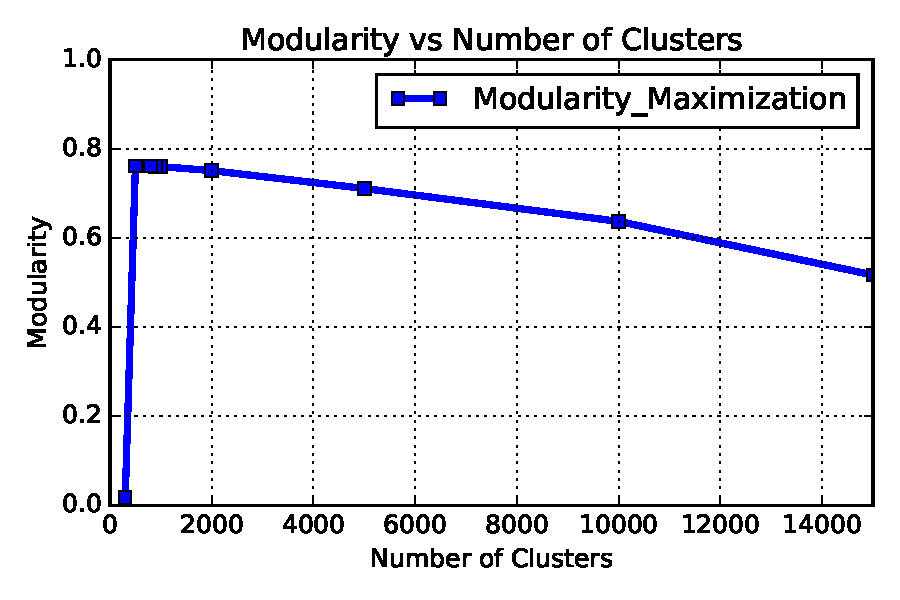
\includegraphics[width = 2in]{../Figures/Modularity_Maximization_modularity_score_whole.pdf}\label{fig:modularity_whole_a}}
  	\subfloat[][Cluster size distribution.]{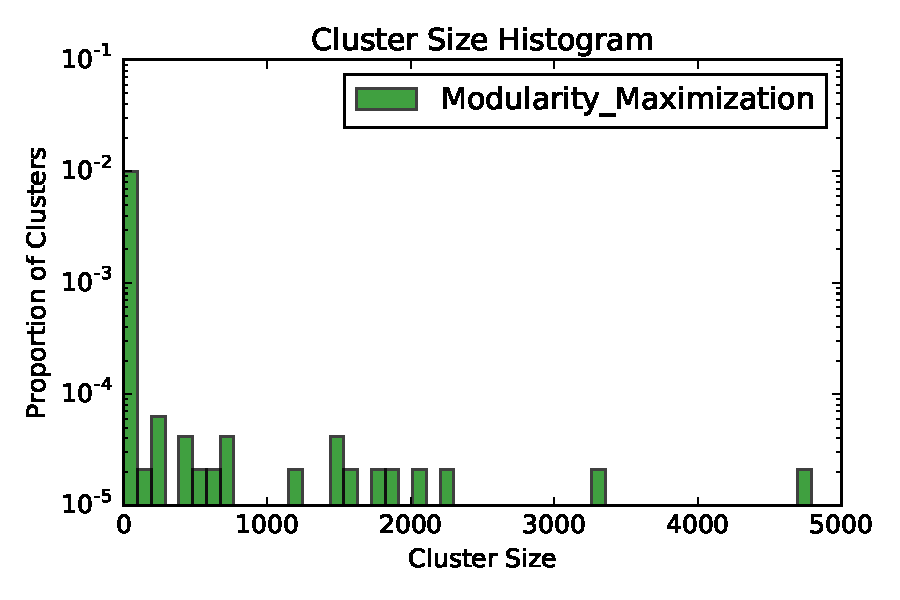
\includegraphics[width = 2in]{../Figures/Modularity_Maximization_cluster_size_whole.pdf}\label{fig:modularity_whole_b}}
  	\subfloat[h][Network of Clusters.]{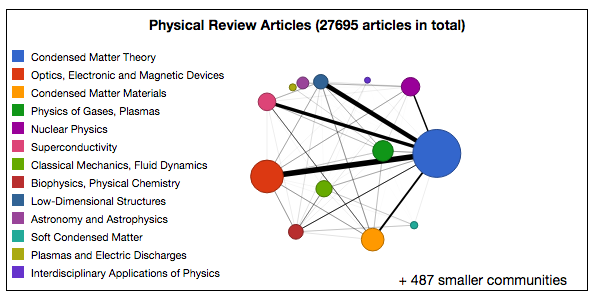
\includegraphics[width = 1.5in]{../Figures/visualization_whole.png}\label{fig:modularity_whole_c}}
 	\caption{The modularity function, the cluster size distribution function, and the resulting cluster network in the simulation with the agglomerative modularity maximization algorithm on the whole network.}
 	\vspace{-10pt}
  \label{fig:modularity_whole}
\end{figure}

\section{Discussion and Conclusions}

The agglomerative modularity maximization clustering has performed well for a network of citations between more than twenty-thousand physics articles. The resulting community structure corresponds closely to the research groups in the field. The modularity of the final clustering has a peak at $Q=0.762$, which is rather high in real world networks. This indicates strong community structure in the physics world. One could try to follow each individual community to observe how they break up. One can also perform the time evolution of the community structure by splitting the citation network according to different periods of time. 

\small{
\begin{thebibliography}{9}
\bibitem{phys_rev}
P. Chen, S. Redner. \textit{Community structure of the physical review citation network}, Journal of Informetrics, {\bf 4} (2010) 278-290.

\bibitem{OLED}
Y. Kajikawa, Y. Takeda. \textit{Citation network analysis of organic LEDs}, Technological Forecasting and Social Change, {\bf 76} (2009) 1115-1123.

\bibitem{learning_analytics}
S. Dawson, D. Gasevic, G. Siemens, S. Joksimovic. \textit{Current State and Future Trends: A Citation Network Analysis of the Learning Analytics Field}, In Proceedings of the Fourth International Conference on Learning Analytics And Knowledge (LAK 2014). ACM, New York, NY, USA, 231-240.

\bibitem{sustain}
Y. Kajikawa, J. Ohno, Y. Takeda, K. Matsushima, H. Komiyama. \textit{Creating an academic landscape of sustainability science: an analysis of the citation network}, Sustain Science, (2007) {\bf 2}:221-231.

\bibitem{Newman_divisive} E. A. Leicht, and M. E. J. Newman. \textit{Community structure in directed networks}, Physical Review Letters, (2008) {\bf 100}, 118703.

\bibitem{bottom_up} V. D. Blondel, J. L. Guillaume, R. Lambiotte, and E. Lefebvre, E. (2008). \textit{Fast unfolding of communites in large networks}, Journal of Statistical Mechanics: Theory and Experiment, P1008, 1742–5468.

\bibitem{new_method}
P. Zhao, and C. Zhang. \textit{A new clustering method and its application in social networks}, Pattern Recognition Letters {\bf 32} (2011) 2109-2118.

\bibitem{Newman_evaluation}
M. E. J. Newman, and M. Girvan. \textit{Finding and evaluating community structure in networks}, Phys. Rev. E {\bf 69}, 026113 (2004).

\bibitem{method_review}
L. Danon, A. Diaz-Guilera, J. Duch, and A. Arenas. \textit{Comparing community structure identification}, J. Stat. Mech. (2005) P09008.

\bibitem{Newman_algorithm}
M. E. J. Newman. \textit{Fast algorithm for detecting community structure in networks}, Phys. Rev. E {\bf 69}, 066133 (2004).

\end{thebibliography}
}

\end{document}
